\documentclass[letterpaper]{article}


\usepackage{amsmath,amsfonts,amsthm} % Math packages
%\usepackage[margin = 1in]{geometry}
\usepackage{tikz} %for the GUI
\usepackage{graphicx}
\usepackage{todonotes}
\usepackage{listings}

\lstdefinestyle{base}{
  breaklines=true,
  basicstyle=\ttfamily\color{black},
  moredelim=**[is][\color{red}]{@}{@},
}

\begin{document}

\section{Ideas}

\subsection{Initial}


\begin{itemize}
   \item Purchase Raspberry Pi Zero
   \item Purchase Nordic Semiconductor ANT+ chip\todo[color=green]{The more I think about it, the more I think we need to use the dongle...}
   \item General steps\todo{any thoughts on this procedure?}\todo[color=green]{We should try to find ways to work simultaneously on different things to make things smoother. Fewer merges, etc.}
   \begin{enumerate}
      \item Purchase ANT+ Chip
      \item Work to adapt a C++ ANT+ library to receive data stream from peripheral devices
      \item Implement calculations and cycling features
      \item Design the user interface using QT Creator\todo[color=green]{QT looks like a pain. Evaluate other options, Tkinter?}
      \item Assemble the hardware  
   \end{enumerate}
\end{itemize}

\subsection{Python-ant setup help}
Here is what I did; I hope it works for you. 
\begin{enumerate}
   \item Plug in your ant+ dongle and ssh or open command line on device and run. 
      \begin{lstlisting}[frame=single,style=base]
lsusb
      \end{lstlisting}
   \item You should find a device along the lines of \texttt{Dynastream Innovations, Inc. Mini stick Suunto}. Take note of the vendor ID and product ID. They are probably \texttt{0fcf} and \texttt{1008} respectively. 
   \item We need a node to be created as a static way to refer to the USB device if it is plugged in. To do this, we create a rule using the following command, but be sure you have the ant+ stick removed. 
   \begin{lstlisting}[frame=single,style=base]
sudo vi /etc/udev/rules.d/garmin-ant2.rules
   \end{lstlisting}
   Copy and paste this stuff to the file but change the red stuff if your vendor ID and product ID are different.
   \begin{lstlisting}[frame=single,style=base]
SUBSYSTEM=="usb", ATTRS{idVendor}=="@0fcf@", ATTRS{idProduct}=="@1008@", RUN+="/sbin/modprobe usbserial vendor=@0x0fcf@ product=@0x1008@", MODE="0666", OWNER="pi", GROUP="root"
   \end{lstlisting}
   \item Plug the movestick back in and check \texttt{/dev} for \texttt{ttyUSB0}.
   \item Next are some dependencies and random stuff you need. 
   \begin{lstlisting}[frame=single,style=base]
git clone https://github.com/baderj/python-ant.git
sudo apt-get install -y python-setuptools
cd python-ant/
sudo python setup.py install
   \end{lstlisting}
   \item To test that everything is working. Look in \texttt{demos/ant.core} and run 
   \begin{lstlisting}[frame=single,style=base]
python 04-processevents.py 
   \end{lstlisting}


\end{enumerate}
      

\section{Features}
\begin{itemize}
   \item CP curve
   \begin{itemize}
      \item Curve fit
      \item Data file with best power for ever interval
   \end{itemize}
   \item W' implementation
\end{itemize}



\section{Screen Choice}
On screen choice, I think it will decide how we interact with the device. Basically, whether or not it is a touch screen. An additional note: displays can interact with an RPi with either the GPIO pins or a serial display output. I think we need to use the serial display output to free up the GPIO for any other devices. The touch screen I have uses GPIO which would make this hard. 

\begin{itemize}
   \item Touch screen\todo{do you know if any units have touch screen and buttons? actually i think the pioneer head unit does.. maybe EDGE 510 as well? have to look how touch screen perform when sweat/wet}\todo[color=green]{I think 510 has both. I think we can do JUST touch screen. Resistive touch screen has no problem with sweat.}.
      \begin{itemize}
         \item Resistive
         \item Capacitive - \textbf{NO}
      \end{itemize}
   \item Just normal screen with buttons
\end{itemize}

\section{Graphical User Interface}

\begin{figure}[!htb]
\centering
\begin{minipage}{.49\textwidth}
\centering
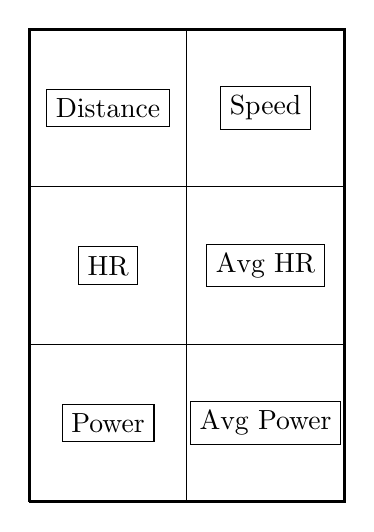
\begin{tikzpicture}
\draw[very thick] (0,0) -- (4,0) -- (4,6) -- (0,6) -- (0,0);
\draw (0,2) -- (4,2);
\draw (0,4) -- (4,4);
\draw (2,0) -- (2,6);
\node[draw] at (1,1) {Power};
\node[draw] at (3,1) {Avg Power};
\node[draw] at (1,3) {HR};
\node[draw] at (3,3) {Avg HR};
\node[draw] at (1,5) {Distance};
\node[draw] at (3,5) {Speed};
\end{tikzpicture}

\caption{Home page}
\end{minipage} \hfill
\begin{minipage}{.49\textwidth}
\centering
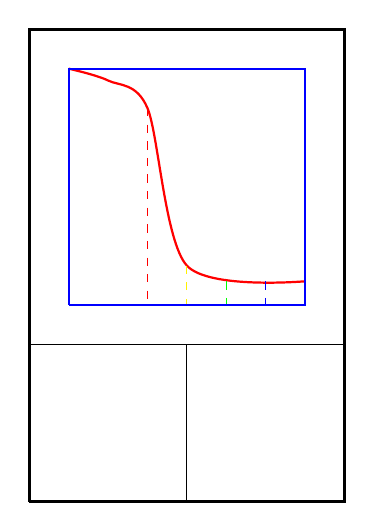
\begin{tikzpicture}
\draw[very thick] (0,0) -- (4,0) -- (4,6) -- (0,6) -- (0,0);
\draw (0,2) -- (4,2);
\draw (2,0) -- (2,2);
\draw [red,thick] plot [smooth] coordinates {(.5,5.5) (1,5.35) (1.5,5) (2,3) (3.5,2.8)};
\draw[dashed,red] (1.5,5) -- (1.5, 2.5);
\draw[dashed,yellow] (2,3) -- (2, 2.5);
\draw[dashed,green] (2.5,2.8) -- (2.5, 2.5);
\draw[dashed,blue] (3,2.8) -- (3, 2.5);
\draw[blue, thick] (.5,2.5) -- (3.5,2.5) -- (3.5,5.5) -- (.5,5.5) -- (.5,2.5);
\end{tikzpicture}

\caption{CP}
\end{minipage}
\end{figure}

\end{document}
